\chapter{Evaluation}\label{chap:eval}

A user study was conducted to evaluate Replico's efficiency, effectiveness, and user-friendliness. The main goal was determining how easily users could communicate points of interest within the virtual environment using Replico. Secondary goals included assessing ease of use and overall user experience. The study aimed to answer four key research questions:

\begin{itemize}
    \item \textbf{RQ1}: How efficiently can users create a point of interest on a given object?
    \item \textbf{RQ2}: How effectively does Replico notify users when a point of interest is created?
    \item \textbf{RQ3}: How useful is the world-in-miniature metaphor for communicating points of interest? How useful is the representation of user locations on the replica for understanding intent? % 2nd part is inconclusive, users didn't use it :(
    \item \textbf{RQ4}: How user-friendly is Replico, and how much physical effort is required to use it? 
\end{itemize}

\section{Setup}

    % TODO: get computer specs

    The user study was conducted at FEUP, in the GIG laboratory in room I220. The setup included two VR-ready computers connected to a local network. Each computer had an HTC Vive Pro 2 headset and a VR controller for table tracking. Two touch surfaces -- a 32-inch infrared frame and a 47-inch capacitive Displax Skin Ultra touchscreen -- were placed on opposite tables within the central VR play space. Participants, in pairs, were seated in front of each touch surface with their backs facing each other, as shown in Figure \ref{fig:eval_setup}.

    \begin{figure}[h]
        \centering
        \includegraphics[width=1\linewidth]{figures/setup.png}
        \caption{Setup for the user study. In image (a) one participant is seated in front of the Displax Skin Ultra. In image (b) the participant is seated in front of the infrared touch frame.}
        \label{fig:eval_setup}
    \end{figure}

    One computer served as the host, while the other connected as a client. The setup process involved a starting screen where the moderator could select the IP address of the host computer. The roles of each computer did not change throughout the study to simplify the setup process and avoid confusion.

\section{Methodology}

    The study was conducted in pairs, with initial tasks performed individually and later tasks performed collaboratively. Each session consisted of three main parts: an introduction, a training session, and the main tasks. Each session lasted approximately 60 minutes. After each session, participants received a chocolate bar as a token of appreciation.

    Before the study began, participants were introduced briefly to the study's purpose and the Replico system. They then completed a consent form and a profiling questionnaire. Following this, they watched a video presentation explaining Replico's features, usage, and the tasks they would perform.

    During the training session, participants familiarized themselves with the system by experimenting with all of Replico's features. Once comfortable with the solo interactions, a set of points of interest and a simulated player were added to the environment, allowing users to practice acknowledging points of interest and joining the other user's table. After becoming comfortable with these interactions, they proceeded to the main tasks.

    The main tasks were performed using two different 3D models: a city and the Perseverance rover, described in Section \ref{sec:test_scenarios}. The order in which the models were used alternated between pairs to avoid bias. These tasks aimed to assess the efficiency and effectiveness of Replico's features, as described in Section \ref{sec:tasks}. Metrics for each task were collected as detailed in Section \ref{sec:evaluation_metrics}. Participants completed a questionnaire on the tasks they performed between each test scenario, described in Section \ref{sec:qualitative_data}.

    \subsection{Test Scenarios} \label{sec:test_scenarios}

        Three scenarios were used during the study, two for the main tasks, as shown in Figure \ref{fig:test_scenarios}. The first scenario, used for training, is a small dungeon tavern built with the free version of the KayKit Dungeon Remastered Pack from itch.io\footnote{\url{https://kaylousberg.itch.io/kaykit-dungeon-remastered}} and the Modular Asset Staging Tool (MAST) for Unity\footnote{\url{https://fertile-soil-productions.itch.io/mast}}. The second scenario is a city from Synty's POLYGON City Pack\footnote{\url{https://assetstore.unity.com/packages/3d/environments/urban/polygon-city-low-poly-3d-art-by-synty-95214}}, obtained through Unity's student plan. The third scenario features the Perseverance rover, obtained from NASA's 3D model repository\footnote{\url{https://nasa3d.arc.nasa.gov/detail/perseverance-glb}}, with the surrounding environment created using Unity's terrain tools and a tinted sand texture from Polyhaven\footnote{\url{https://polyhaven.com/a/sand_01}}.

        \begin{figure}[h]
            \centering
            \includegraphics[width=1\linewidth]{figures/test_scenarios.png}
            \caption{The three test scenarios used in the user study. From left to right: the dungeon tavern, the city, and the Perseverance rover.}
            \label{fig:test_scenarios}
        \end{figure}

        Two scenarios were selected for the main tasks to evaluate how well the approach works with different 3D models. The city model was chosen for its large, complex structure, allowing users to immerse themselves within it. The Perseverance rover model was selected for its smaller size but sufficient detail, enabling users to view the entire model at once without being part of it. The dungeon tavern was used for practice, providing a small, enclosed environment distinct from the main task scenarios.

        In all scenarios, the virtual world includes surrounding environment elements to provide context and a sense of scale. For example, the city is bordered by an ocean, the rover by the Martian surface, and the dungeon tavern by some of its walls. The WIM does not replicate these environmental elements, as they are not part of the primary scenario.

    \subsection{Tasks} \label{sec:tasks}

        Participants performed five main tasks during the study, using each of the two main scenarios. The first three tasks were done individually, while the last two were collaborative. Each task evaluated different aspects of Replico's features and user experience. The tasks are as follows:

        \begin{itemize}
            \item \textbf{Task 1}: Create a point of interest on six different predefined objects in the scene. This task evaluates how efficiently users can create points of interest.
            \item \textbf{Task 2}: Acknowledge five out of twelve predefined points of interest created by a simulated user. This task assesses how effectively Replico notifies users of new points of interest.
            \item \textbf{Task 3}: Teleport to four different predefined zones and orient themselves to face a specific object. This task measures how well users can navigate the environment using Replico.
            \item \textbf{Task 4 \& 5}: One user must show another user a specific object in the scene without verbal communication. The other user then verbally confirms the object they believe the first user is referring to. Once confirmed, the roles are reversed, and the process is repeated with a different object. This task evaluates how well users can communicate points of interest using Replico
        \end{itemize}

        Between each task, the environment was reset to its initial state. This meant that any points of interest created during the previous task were removed, and participants were placed back at their starting positions. This was done to ensure that each task was performed under the same conditions for all participants.

        In the first task, the predefined objects were chosen with different sizes and at various heights, visible in Figure \ref{fig:task_01}. The goal was to evaluate how efficiently users could create points of interest, not to test their ability to identify objects. To draw attention to them, these objects glowed with an expanding and contracting effect in the WIM. They increased in size and changed their outline color from white to green when the balloon intersected with them. Creating a point of interest during this state allowed users to progress to the next object. The objects appeared one at a time, immediately after the user created a point of interest on the previous object. The order in which the objects appeared was consistent for all participants.

        \begin{figure}[h!]
            \centering
            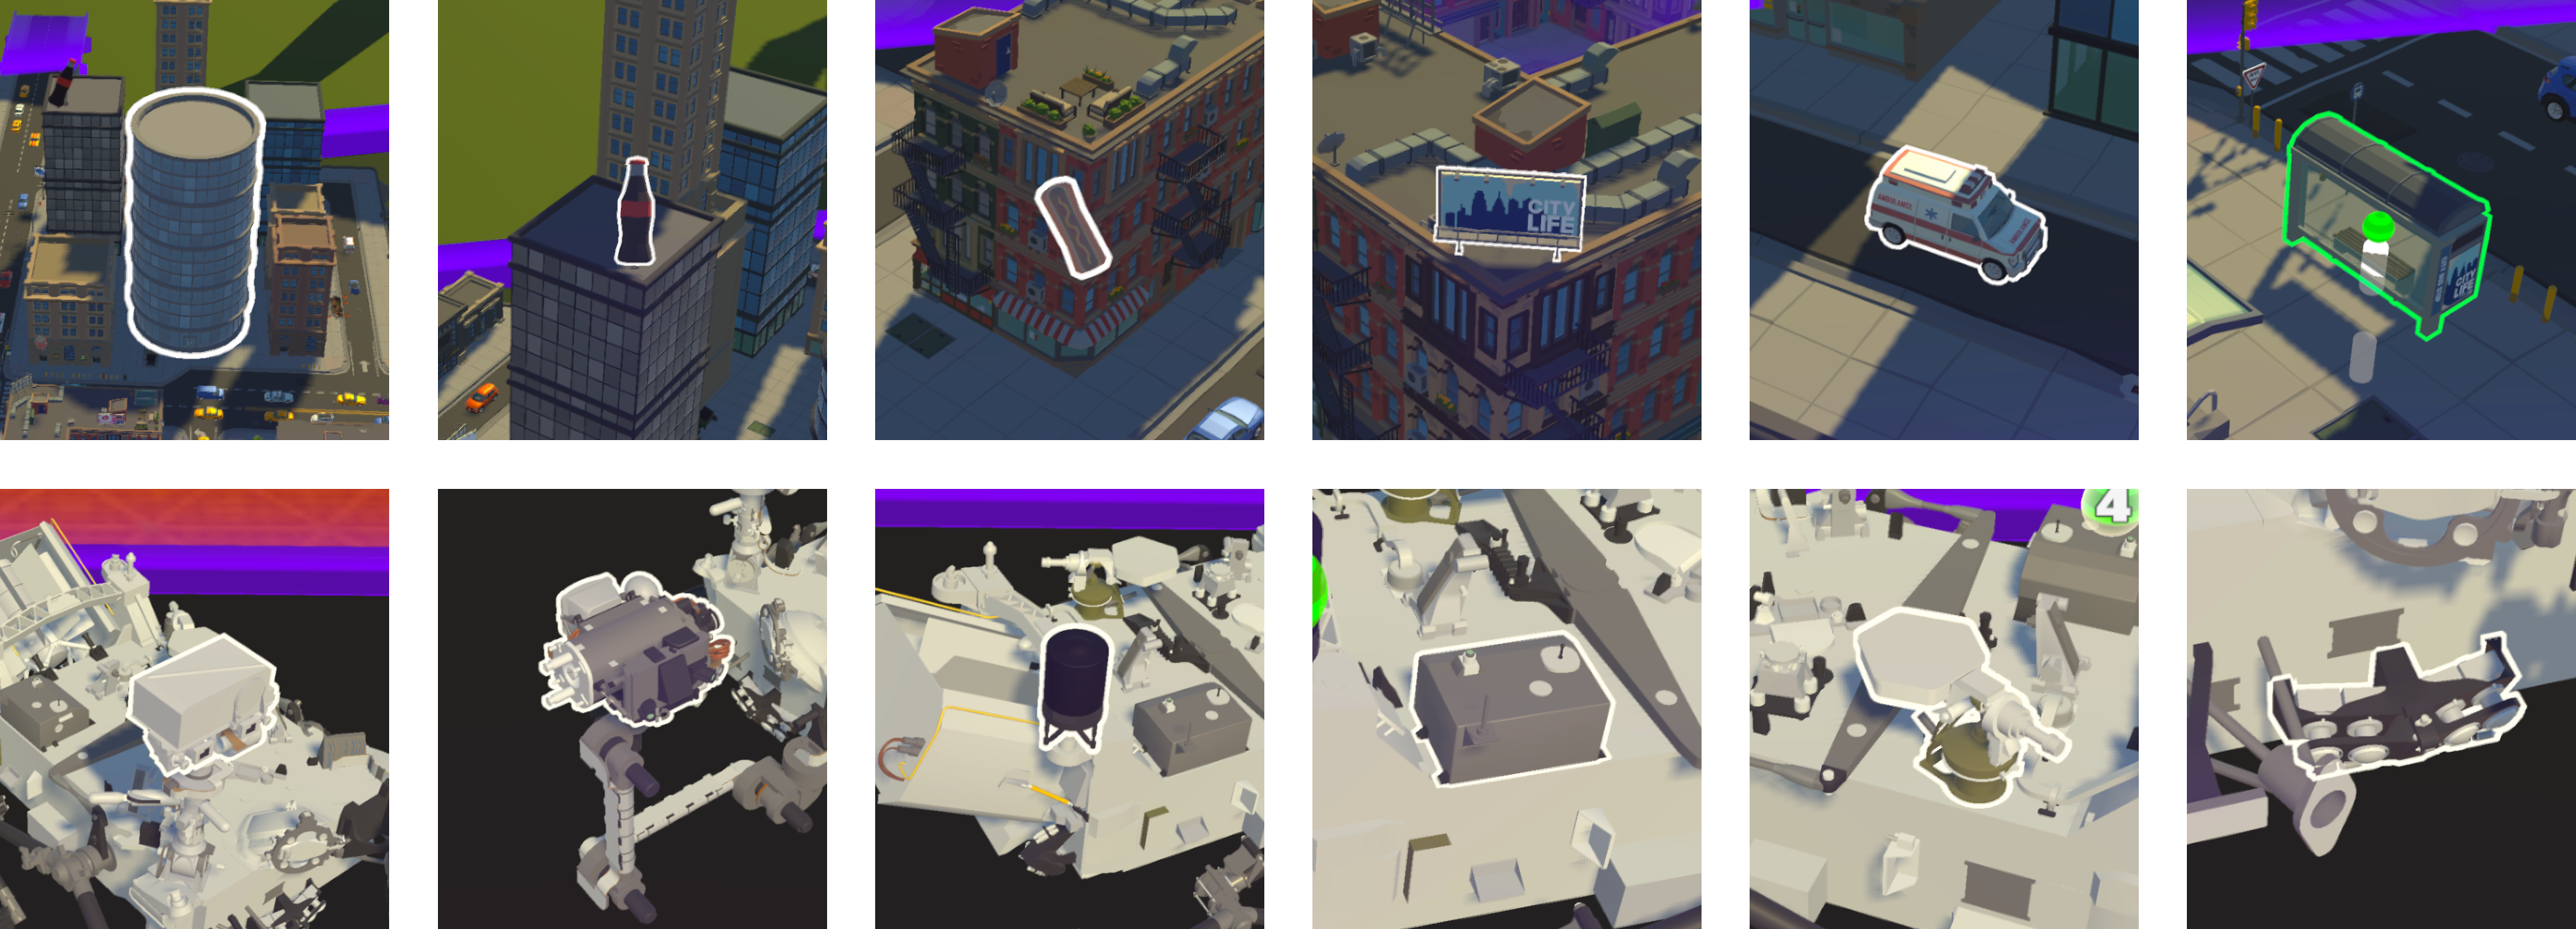
\includegraphics[width=1\linewidth]{figures/task_01.png}
            \caption{The six predefined objects used in Task 1 for each scenario. They are ordered from left to right, with the top row showing the objects in the city scenario while the bottom row shows the objects in the Perseverance rover scenario. The top-right image shows the green outline effect that appears when the balloon intersects with the object.}
            \label{fig:task_01}
        \end{figure}

        In the second task, the predefined points of interest were placed around the environment simultaneously, as shown in Figure \ref{fig:task_02}. The goal was to evaluate how effectively Replico notifies users of new points of interest and helps distinguish acknowledged from unacknowledged points of interest. The task was complete when the user acknowledged the five unacknowledged points of interest. Participants could acknowledge the points of interest in any order.

        \begin{figure}[h!]
            \centering
            \includegraphics[width=1\linewidth]{figures/task_02.png}
            \caption{The created points of interest in Task 2. Image (a) shows the points of interest in the city scenario, while image (b) shows the points of interest in the Perseverance rover scenario.}
            \label{fig:task_02}
        \end{figure}

        In the third task, participants navigated through four predefined zones in the environment, as shown in Figure \ref{fig:task_03}. The goal was to assess how well users could navigate using Replico. Participants were instructed to teleport to each zone and orient themselves to face a specific object. Zones changed color from white to green when the balloon intersected with them, and the object's glow effect also changed from white to green when the user was correctly oriented. The moderator advanced the task manually, allowing participants to take their time exploring the environment. The sequence of zones was the same for all participants.

        \begin{figure}[h]
            \centering
            \includegraphics[width=1\linewidth]{figures/task_03.png}
            \caption{The four predefined zones used in Task 3 for each scenario. They are ordered from left to right, with the top row showing the zones in the city scenario while the bottom row shows the zones in the Perseverance rover scenario.}
            \label{fig:task_03}
        \end{figure}

        In the fourth and fifth tasks, participants communicated objects of interest without verbal communication. Figure \ref{fig:task_04} shows the objects used in these tasks. The goal was to assess how effectively users could communicate using Replico. The selected objects were small and difficult to identify from a distance, encouraging the use of the WIM, points of interest, and teleportation for effective communication. For the Perseverance rover model, since most people are unfamiliar with its components, the objects chosen were a small hidden star and a small hidden heart.

        \begin{figure}[h]
            \centering
            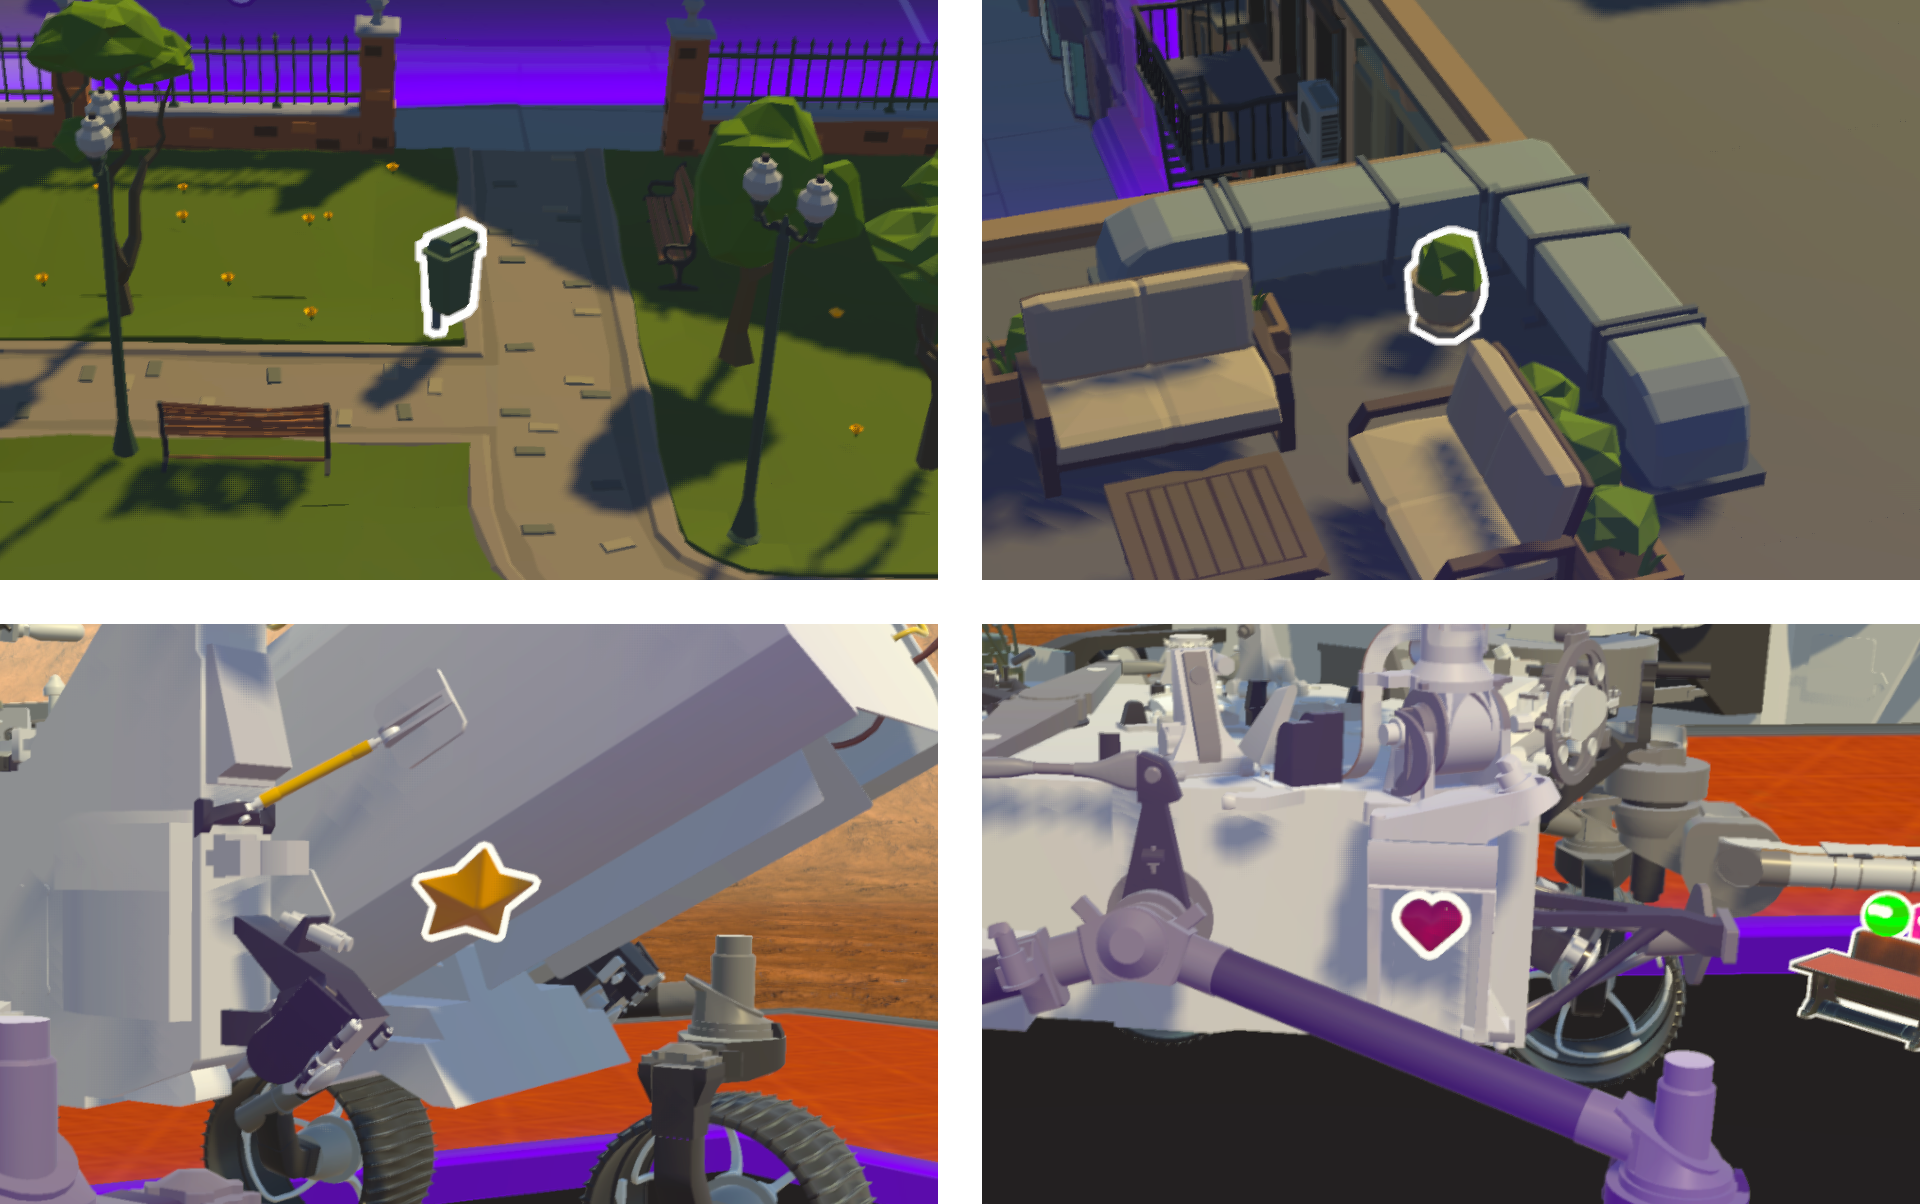
\includegraphics[width=1\linewidth]{figures/task_04.png}
            \caption{The objects used in Tasks 4 and 5 for each scenario. The top row shows the objects in the city scenario, while the bottom row shows the objects in the Perseverance rover scenario.}
            \label{fig:task_04}
        \end{figure}


    \subsection{Metrics} \label{sec:evaluation_metrics}

        During each task, several metrics were collected to evaluate the efficiency and effectiveness of Replico's features. 

    \subsection{Qualitative Data} \label{sec:qualitative_data}

% do speak about how the frame being too sensitive to resting arms impacted the results